\documentclass[../../main.tex]{subfiles}

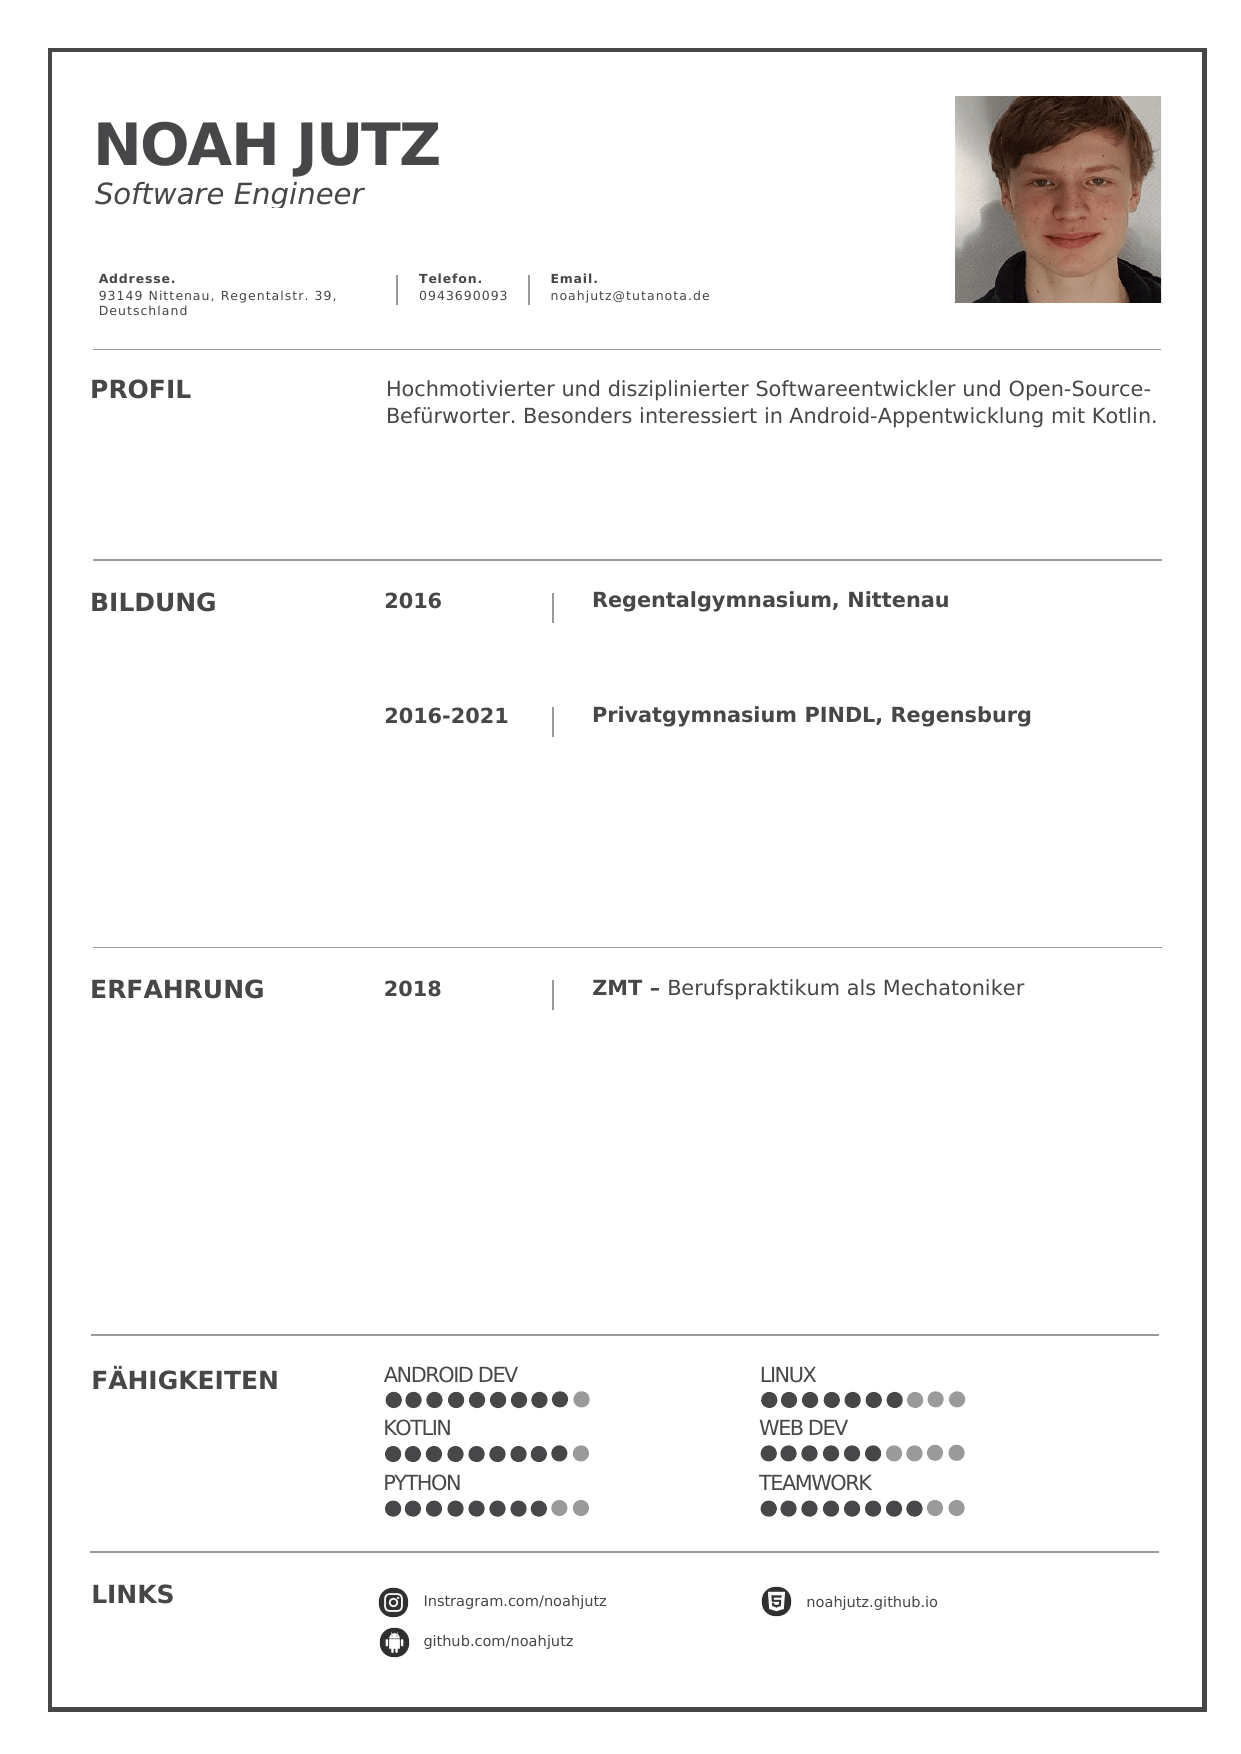
\includegraphics[width=\textwidth]{cv.png}

\noindent Noah Jutz
\newline Regentalstraße 39
\newline 93149 Nittenau
\newline noahjutz@tutanota.de
\newline

\noindent Tutanota
\newline Deisterstr. 17a
\newline 30449 Hanover
\newline jobs@tutao.de
\newline

\begin{flushright}
    2020-12-07
\end{flushright}

\noindent \textbf{Bewerbung als Softwareentwickler}
\newline

\noindent Sehr geehrte Damen und Herren,
\newline

\noindent Nachdem ich Tutanota auf Tutanota als Email-Anbieter umgestiegen bin, ist zu meiner Aufmerksamkeit gekommen, dass Sie offene Stellen für Softwareentwickler haben. Weil ich mit meinen Programmierkenntnissen Positives bewirken will und mir Online-Privatsphäre besonders am Herzen liegt, habe ich mich entschieden, mich bei Ihnen zu bewerben. Mit meinen Fähigkeiten Ihren Open-Source-Projekten beizutragen wäre mir eine große Freude.

Ich bin ein motivierter und disziplinierter Softwareentwickler mit Schwerpunkt auf Android. Mit einem Jahr Erfahrung mit Kotlin Android-Development kenne ich mich mit den gängigsten Frameworks (Darunter Jetpack Compose, Room, Hilt, etc.) und Programmierdenkmustern aus, und verfüge darüber hinaus die Fähigkeit logischem Denkens. Diese Fertigkeiten habe ich mit meinem persönlichem Projekt einer Open-Source Fitness-App ``GymRoutines'' unter Beweis gestellt.

Ich freue mich über ein persönliches Interview.
\newline

\noindent Mit freundlichen Grüßen

\noindent Noah Jutz